\renewcommand{\theequation}{\theenumi}
\begin{enumerate}[label=\thesection.\arabic*.,ref=\thesection.\theenumi]
\numberwithin{equation}{enumi}
%
\item
\label{ch2_constraint}
Modify the code in problem \ref{convex_code} to find a graphical solution for minimising
\begin{align}
f\brak{\mbf{x}} 
%= (x_1-8)^2 + (x_2-6)^2
\end{align}
with constraint
\begin{align}
%\label{convex-constraint}
g\brak{\mbf{x}} \geq 0
%= x_1 + x_2 - 9 
\end{align}

\solution 
This problem reduces to finding the radius of the smallest circle in the shaded area in Fig. \ref{fig.2.4} .  It is clear that this radius is 0.
%	
\begin{lstlisting}
opt/codes/2.4.py
\end{lstlisting}

%
\begin{figure}[!ht]
\centering
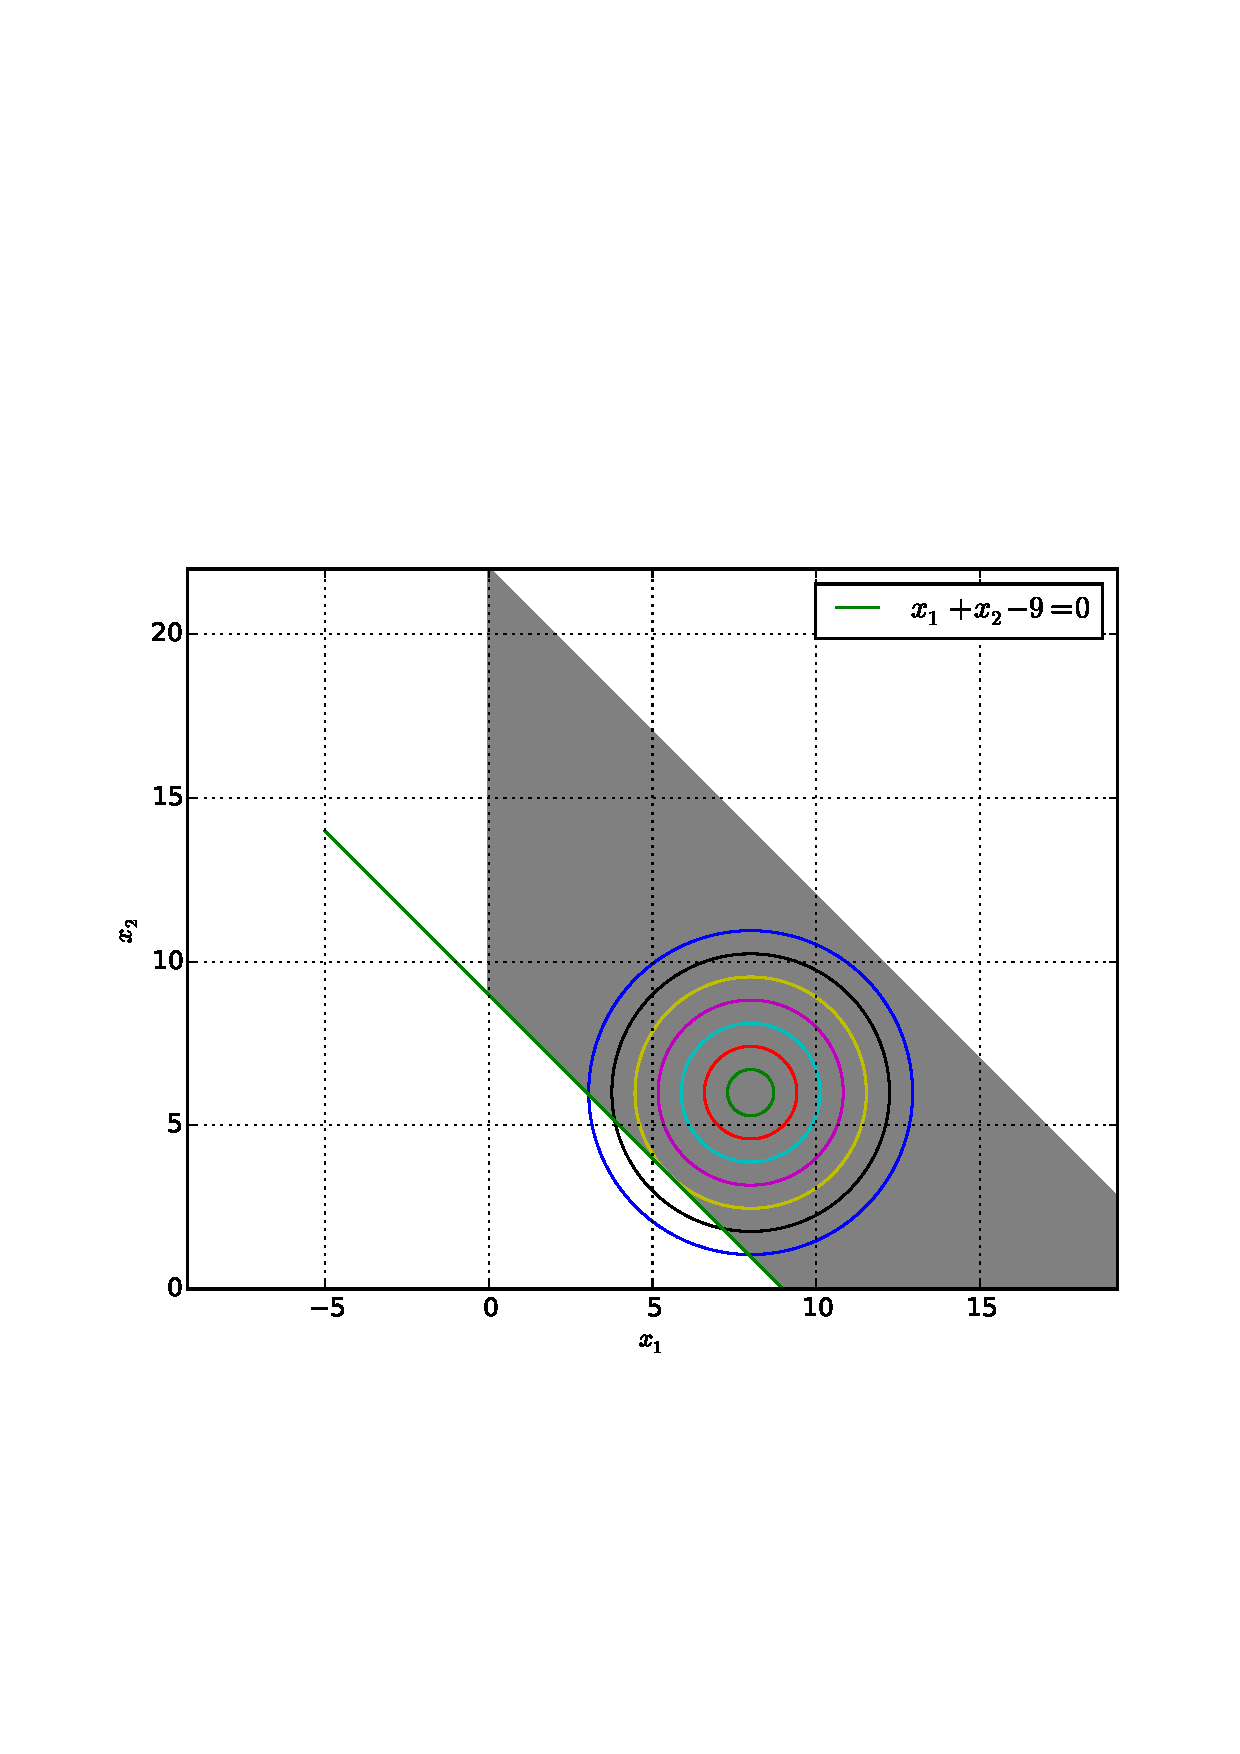
\includegraphics[width=\columnwidth]{./opt/figs/2.4.png}
\caption{ Smallest circle in the shaded region is a point.}
\label{fig.2.4}	
\end{figure}
%
\item
\label{ch2_lagrange_fail}
Now use the method of Lagrange multipliers to solve  problem \ref{ch2_constraint} and compare with the graphical solution.  Comment.

%
\solution Using the method of Lagrange multipliers, the solution is the same as the one obtained in  problem \ref{ch2_constraint}, which is different from the graphical solution.  This means that the Lagrange multipliers method cannot be applied blindly.
\item
Repeat problem \ref{ch2_lagrange_fail} by keeping 
 $\lambda=0$.   Comment.

\solution Keeping $\lambda = 0$ results in $\vec{x}=\myvec{ 3\\ -5}$, which is the correct solution.  The minimum value of $f\brak{\mbf{x}}$ without any constraints lies in the region $g\brak{\mbf{x}} = 0$.  In this case, $\lambda = 0$.  
%
%
\item
\label{ch2_constraint_border}
Find a graphical solution for minimising
\begin{align}
f\brak{\mbf{x}}
% = (x_1-8)^2 + (x_2-6)^2
\end{align}
with constraint
\begin{align}
%\label{convex-constraint}
g\brak{\mbf{x}} \leq 0
%= x_1 + x_2 - 9 .
\end{align}
Summarize your observations.

\end{enumerate}
\iffalse
%
\solution In Fig. \ref{fig.2.7}, the shaded region represents the constraint.  Thus, the solution is the same as the one in problem \ref{ch2_constraint}. This implies that the method of
Lagrange multipliers can be used to solve the optimization problem with this inequality constraint as well.  Table \ref{table.2.7} summarizes the conditions for this based on the observations so far.
\begin{lstlisting}
wget https://raw.githubusercontent.com/gadepall/optimization/master/opt/codes/2.7.py
\end{lstlisting}

%
\begin{figure}[!ht]
\centering
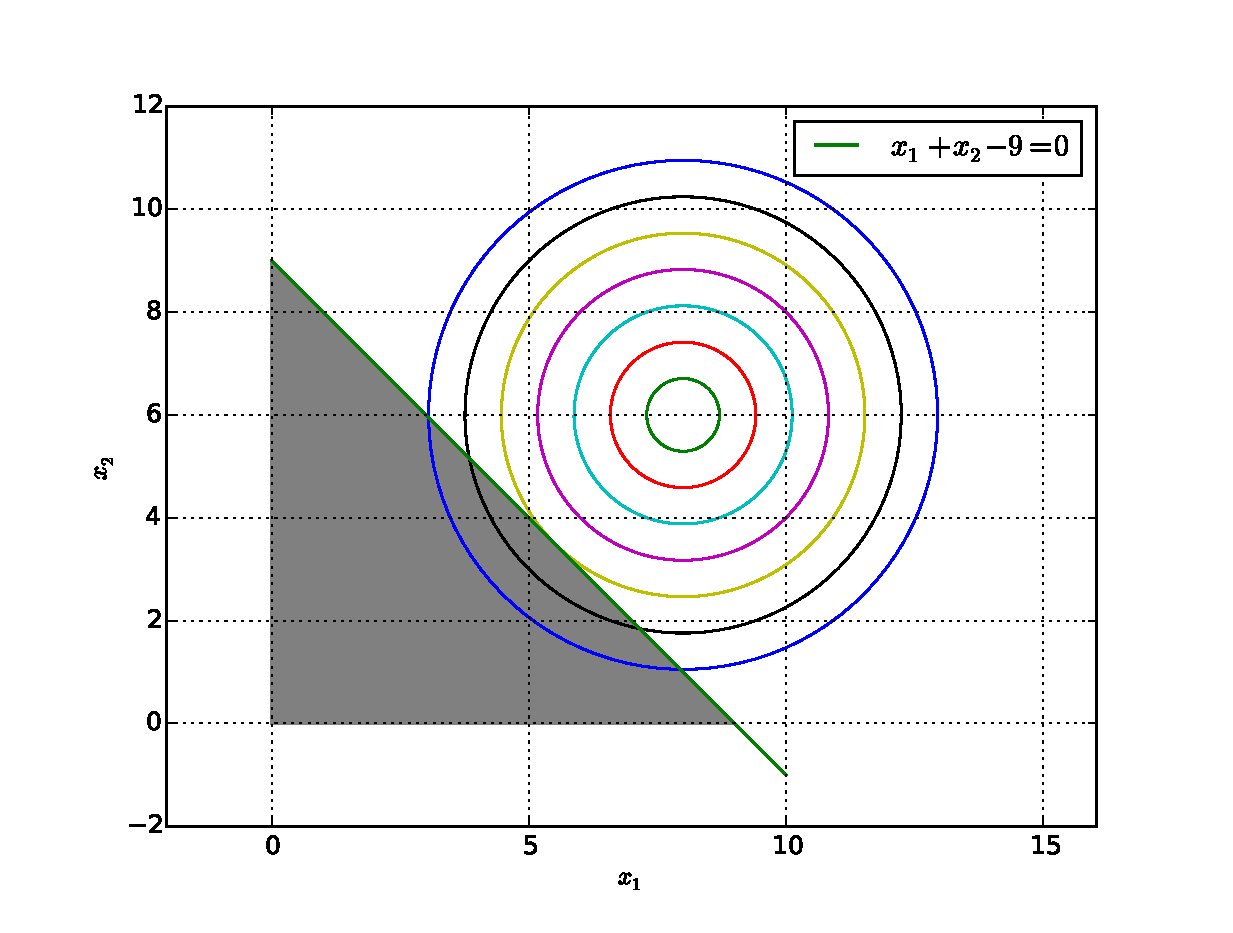
\includegraphics[width=\columnwidth]{./opt/figs/2.7.eps}
\caption{ Finding $ \displaystyle \min_{\mbf{x}}f\brak{\mbf{x}}$.}
\label{fig.2.7}	
\end{figure}
\input{./opt/figs/tab.2.7.tex}
%
\item
\label{ch2_prob_upper}
Find a graphical solution for 	 
	 \begin{align}
	 \label{ch2_second_min}
	\min_{\mbf{x}} f\brak{\mbf{x}} = \norm{\vec{x}-\myvec{8\\6}}^2
	 \end{align}
	 with constraint
	 \begin{align}
	 \label{ch2_second_const}
	 g\brak{\mbf{x}} = \myvec{1 & 1}\vec{x} - 18 = 0
	 \end{align}
	 
%
\solution
%	
\begin{lstlisting}
wget https://raw.githubusercontent.com/gadepall/optimization/master/opt/codes/2.8.py
\end{lstlisting}

%
\begin{figure}[!ht]
\centering
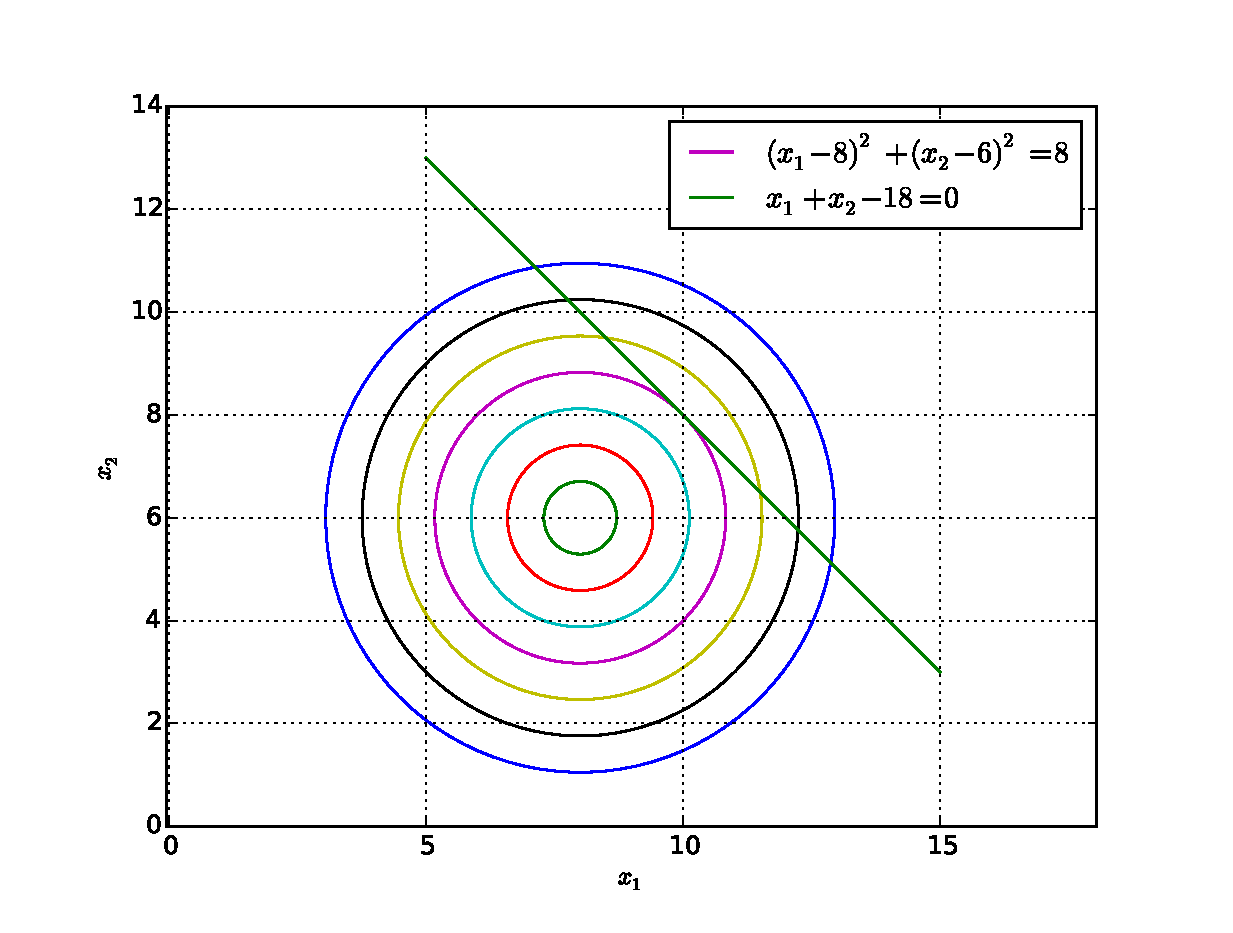
\includegraphics[width=\columnwidth]{./opt/figs/2.8.eps}
\caption{ Finding $ \displaystyle \min_{\mbf{x}}f\brak{\mbf{x}}$.}
\label{fig.2.8}	
\end{figure}
%
\item
Repeat problem \ref{ch2_prob_upper} using the method of Lagrange mutipliers.  What is the sign of $\lambda$?

%
\solution
%From \eqref{ch2_second_min} and \eqref{ch2_second_const}, 
%%
%\begin{align}
%L\brak{\mbf{x},\lambda} &= (x_1-8)^2 + (x_2-6)^2 - \lambda \brak{x_1 + x_2 - 18} \\
%\Rightarrow \nabla L\brak{\mbf{x},\lambda}  & = 
%\begin{pmatrix}
%2x_1  - 16 - \lambda \\
%2x_2 - 12 - \lambda \\
%x_1 + x_2 -18
%\end{pmatrix}
%\\
%&=
%\begin{pmatrix}
%2 &0 & - 1 \\
%0 &2 & - 1 \\
%1 & 1 & 0 
%\end{pmatrix}
%\begin{pmatrix}
%x_1 \\
%x_2 \\
%\lambda
%\end{pmatrix}
%= 
%\begin{pmatrix}
%16 \\
% 12 \\
%18
%\end{pmatrix}
%=
%0 
%\\
%\Rightarrow 
%\begin{pmatrix}
%x_1 \\
%x_2 \\
%\lambda
%\end{pmatrix}
%&= 
%\begin{pmatrix}
%10 \\
% 8 \\
%4
%\end{pmatrix}
%\end{align}
%%
Using the following python script, $\lambda$ is positive and the minimum value of $f$ is 8.
%	
\begin{lstlisting}
wget https://raw.githubusercontent.com/gadepall/optimization/master/opt/codes/2.9.py
\end{lstlisting}

%
%
\item
\label{ch2_prob_upper_cond}
Solve
	 \begin{align}
%	 \label{ch2_second_min}
	\min_{\mbf{x}} f\brak{\mbf{x}} 
%= (x_1-8)^2 + (x_2-6)^2
	 \end{align}
	 with constraint
	 \begin{align}
%	 \label{ch2_second_const}
	 g\brak{\mbf{x}} 
%= x_1 + x_2 - 18 
\geq 0 
	 \end{align}
	 
%
\solution Since the unconstrained solution is outside the region $g\brak{\mbf{x}} \geq 0$, the solution is the same as the one in problem \ref{ch2_prob_upper}.
%
\item
Based on the problems so far, generalise the Lagrange multipliers method for 
%
	 \begin{align}
	 \label{ch2_lagrange_ineq}
	\min_{\mbf{x}} f\brak{\mbf{x}} , \quad 
	 g\brak{\mbf{x}}  \geq 0 
	 \end{align}
%

%
\solution
Considering $L\brak{\mbf{x},\lambda} = f\brak{\mbf{x}} - \lambda g\brak{\mbf{x}}$, for $g\brak{\mbf{x}} = \myvec{1 & 1}\vec{x} - 18 \geq 0$ we found $\lambda > 0 $ and for $g\brak{\mbf{x}} = \myvec{1 & 1}\vec{x} - 9 \leq 0, \lambda < 0$. A single condition can be obtained by framing the optimization problem as
%
	 \begin{align}
	 \label{ch2_lagrange_ineq_summary}
	\min_{\mbf{x}} f\brak{\mbf{x}} , \quad 
	 g\brak{\mbf{x}}  \leq 0 
	 \end{align}
%
with the Lagrangian
%
\begin{equation}
%\label{ch2_kkt_necessary}
L\brak{\mbf{x},\lambda} = f\brak{\mbf{x}} + \lambda g\brak{\mbf{x}}, %\quad  \lambda > 0,  g\brak{\mbf{x}} \leq 0.
\end{equation}
%
provided
%
\begin{equation}
\label{ch2_kkt_necessary}
\nabla L\brak{\mbf{x},\lambda} = 0 \Rightarrow \lambda > 0
\end{equation}
else, $\lambda = 0$.
\fi
